\begin{task}{3, Implementation of knowledge-based model (20\%)}
In this task our goal is to implement the knowledge-based model mentioned in paper \cite{tordeux2020prediction}. Specifically this model is the parametric Weidmann fitting model for the fundamental diagram. This is a microscopic speed-based model and hence the speed of a single pedestrian is modeled. Before we start with the implementation, we want to provide a brief primer on fundamental diagrams.

In the context of traffic flow, a fundamental diagram graphically illustrates the relationship between flow, density, and speed. It is used to analyze and understand the behavior of traffic in different conditions. In our case of the Weidmann model it is used to model pedestrian speed and from here on we can draw conclusions on pedestrian flow.

Looking into the original document \cite{weidmann1993transporttechnik} by Weidmann from 1993, we were not able to find the function provided in this paper \cite{tordeux2020prediction}. But on page 62 section 4.3.1 "Leistungsfähigkeit in der Ebene" of the original document \cite{weidmann1993transporttechnik} we did find a similar expression that describes pedestrian speed in a similar non-linear way.

\begin{align}
    v_{F, hi} = v_{F, hf}\cdot\left(1-e^{-\gamma\cdot(\frac{1}{D}-\frac{1}{D_{max}})}\right)\label{exp_weid}
\end{align}

Here in \ref{exp_weid} $v_{F, hi}$ is the speed under a certain density, while $v_{F, hf}$ is the speed under a free situation. Next $D$ describes the current density of the pedestrian, while $D_{max}$ is the maximum density, such that a pedestrian can not move anymore. Additionally there is the calibration constant $\gamma$, which for example would have a different value, when considering pedestrian speeds for stairways.

\paragraph{The Weidmann model} Now that we have seen the original Weidmann model\ref{exp_weid} it turns out that the model presented by Tordeux\cite{tordeux2020prediction} differs from it. The original document uses the pedestrian density $D$ as function parameter, while in this paper\cite{tordeux2020prediction} the mean spacing $\overline{s}_K$ is used. Then, the model is defined by equations \ref{exp_tor}, \ref{exp_mean}.

Recall that the variables are described as follows: Here $\overline{s}_K$ is the mean spacing of the pedestrian to its $K$ closest neighbours. $v_0$ is the speed in a free situation. $l$ is the physical size of the pedestrian and $T$ describes the following time gap with the neighbours. Once again we have to critize the authors as the variables $l$ and $T$ are not further detailed in the paper and it is up to speculation on how they are precisely defined. Furthermore it is also unknown how this Weidmann model was obtained from original expression \ref{exp_weid}, though at least it can be easily verfied that the units of the variables are correct.

In the original model the variables $\gamma, D, D_{max}$ have units $(P/m^2)$, which cancel each other out. Similarly the variables $l, \overline{s}_K$ are in units $(m)$ and cancel out with $v_0$ $(m/s)$ and $T$ $(s)$. In total only $m/s$ remains from $v_0$ and $v_{F, hf}$ in the functions $W(...)$ and $v_{F, hi}$, and both describe a speed.

\paragraph{Fitting the parameters for the Weidmann model} As stated previously our goal is to fit the parameters of the Weidmann model to the dataset used in the paper\cite{tordeux2020prediction}. By fitting the parameters we will be able to use the function $W(...)$ to plot the fundamental diagrams. The difficult part is to find all parameters used by the function \ref{exp_tor}, so that we can estimate the function. As stated in the paper \cite{tordeux2020prediction} section 3.3 the function for the fundamental diagram was obtained after performing least squares fitting using the data on the Weidmann model.

\paragraph{Data preprocessing} Given in our raw dataset we have pedestrian ids, frame ids and $(x,y,z)$ coordinates. In our python notebook \verb|preprocessing.ipynb| we first perform some simple data cleaning, which after cleaning are stored in the folders \verb|Bottleneck_Clean| and \verb|Corridor_Clean|. Here the \verb|transform(...)| function from \verb|utils.data_processing.py| removes the $z$-coordinate, as it serves no purpose and additionally $x,y$-coordinates are scaled to meters from cm.

Next the functions \verb|remove_bottleneck_oob(...)| and \verb|remove_corridor_oob(...)| remove $x,y$-coordinates that are out of bounds for each of the test scenarios. While this step ins't detailed in the paper, we know from the paper that measurements are taken within a well defined area as well as that the $x,y$-coordinates are provided in cm. From here we  conclude that we can remove coordinates that lie outside of the specified measurement area. For the "Bottleneck-Scenario" we removed any coordinate that lies outside of the boundaries for $x\in (0.0,8.0)$ and $y\in (0.0, 1.8)$. Similarly we removed coordinates from the "Corridor-Scenario" whenever the lie outside of $x\in (0.0,6.0)$ and $y\in (0.0, 1.8)$. With the basic data cleaning done we are going to calculate the mean spacing $\overline{s}_K$, speeds $v$ and density $D$. For each pedestrian at each frame. Since the data preprocessing isn't detailed in the paper\cite{tordeux2020prediction}, we tried to follow as closely and reasonably as possible to the paper, though we were not able to achieve the exact same results.

\paragraph{Calculating $\overline{s}_K$} For the calculation of the mean spacing we used $K=10$ neighbours, since the paper states that $K=10$ was the highest reasonable value. The paper does not specify how it treats cases when there are less than 10 nearest neighbours. Here we opted to simply calculate the mean spacing $\overline{s}_K$ using only the available neighbours, if there were any.

In table \ref{Tab:ms} we see the mean value of our calculated mean spacing as well as the standard deviation. Our result differ from the paper\cite{tordeux2020prediction}, but we can also see a similarity, that the bottleneck scenario has a higher mean than the corridor scenario. This is expected, since their data preprocessing is unknown.

\begin{table}[H]
\centering
\begin{tabular}{ |c|c|c| }
\hline
Scenario & mean (our) & mean (paper)\\
\hline
Bottleneck & $0.910\pm 0.272$ & $1.14\pm 0.37$\\
\hline
Corridor & $0.905\pm 0.330$ & $1.03\pm 0.40$\\
\hline
\end{tabular}
\caption{Mean value of spacing}
\label{Tab:ms}
\end{table}

\paragraph{Calculating $v$} For the calculation the speed $v$ we tried 2 different approaches.
\begin{itemize}
    \item In our initial approach (old) we calculate the speed by using the previous frame. This means the speed of a pedestrian during a specific frame is the traveled distance since the last frame. Formally we calculate the euclidean distance between the current position and position of the previous frame. In the special case of the first frame we assume that the pedestrian did not move, hence we set the previous frame position to be the same as first frame position. Bu this method is flawed as calculating speeds on a per frame basis ($1/16$ of a second) and scaling them up by $\times 16$ leads to inaccuracies.
    \item In our main approach we instead follow the approach from the paper, were speeds are obtained by differentiating positions over a second (see \cite{tordeux2020prediction} section 3). In terms of implementation, this means we have to consider 16 frames to calculate speeds for a single frame. This leads to the special case where the first and last 8 frames are undefined. We decided here to instead use the average spead of this pedestrian after calculating the speeds for each frame. Additionally in the case where we have less than 16 frames, we use the initial approach to calculate the speed.
\end{itemize}

In table \ref{Tab:speed} we see the mean value of our calculated speeds. Here we can see a comparison between our two approaches, the initial one being marked as old, and the results from the paper \cite{tordeux2020prediction}. As explained in the previous section our data preprocessing probably differs from the one in the paper and therefore our results are slightly different as expected. But we can also see similarities once again, as the mean speed in the bottleneck scenario is much higher than in the corridor scenario. We also have closer values for the standard deviation in our second approach. The old approach calculated speed over a single frame (1/16s), which causes some speeds to have very high values. This is also reflected in the stndard deviation of the old approach. From those 2 approaches we also learn that the corridor scenario has a much lower speed overall.

\begin{table}[H]
\centering
\begin{tabular}{ |c|c|c|c| }
\hline
Scenario & mean (our) & mean (paper) & mean (our - old) \\
\hline
Bottleneck & $0.554\pm 0.324$ & $0.72\pm 0.34$ & $0.623\pm 0.715$\\
\hline
Corridor & $0.327\pm 0.305$ & $0.35\pm 0.33$ & $0.375\pm 0.332$\\
\hline
\end{tabular}
\caption{Mean value of speed}
\label{Tab:speed}
\end{table}

\paragraph{Calculating $D$}Finally we also decided to calculate the densities $D$ for each frame, though it is expanded to each pedestrian, so it can be assigned to each of them in the dataset. For the density we simply counted the amount of people that are within the measurement area and divided that count by the measurement area. In conclusion the mean spacing $\overline{s}_K$, speed $v$ and density $D$ can all be calculated from the data. These are then appended to the cleaned data, which then form our new cleaned dataset.

In table \ref{Tab:dens} we can see our estimations for density in person per $m^2$. Here we see that the bottleneck scenario overall  has a higher mean for pedestrian density compared to the corridor scenario. Similar to the values from table \ref{Tab:ms}, the mean spacing for bottleneck is higher.

\begin{table}[H]
\centering
\begin{tabular}{ |c|c| }
\hline
Scenario & mean \\
\hline
Bottleneck & $1.895\pm 0.813$\\
\hline
Corridor & $1.656\pm 0.976$\\
\hline
\end{tabular}
\caption{Mean value of density}
\label{Tab:dens}
\end{table}

\paragraph{Estimating $v_0, T, l$} In the next step our goal is to estimate the remaining unknown parameters of the Weidmann model. First we will start with estimating the speed under a free situation $v_0$. Once again the paper \cite{tordeux2020prediction} does not specify more except that it was estimated using least squares fitting, which is a very vague statement. We propose the following methodologies to estimate the speed under a free situation $v_0$.

\begin{enumerate}
    \item The first possible approach is to look into dataset at all instances where the pedestrian density $D$ is low enough or mean-spacing $\overline{s}_K$ alows free movement. The main issue is that we do not know the exact values of $D$ or $\overline{s}_K$ such that this is possible. Thus we can only assume that free movement is possible, when only one pedestrian is observed. To calculate this we would have to look at frames in the dataset where this condition holds. Note that this approach has the downside that we consider very few datapoints. Furthermore we might not be able to accurately calculate the speed $v_0$, because our observations are limited to the measurement area. Nonetheless this approach has the benefit as we are sticking close to the original dataset by calculating the average of the observed speed $v_0$.
    \item The second approach is to use the original Weidmann model \ref{exp_weid}. The advantage of this approach is that we have $\gamma$ and $D_{max}$ given from \cite{weidmann1993transporttechnik}. Using these values we can calculate $v_0$ for each point and get a better estimation for $v_0$ by having access to more datapoints. But on the flipside this model is based originally on the Kladek model\cite{kladek1966geschwindigkeitscharakteristik}, which is a macroscopic speed model, since we are using the overall pedestrian density instead of the mean spacing of a specific pedestrian. using the calculated speed, we then used \verb|scipy.optimize.curve_fitting(...)| to obtain the parameters $T,l$.
    \item For the final approach we also used \verb|scipy.optimize.curve_fitting(...)| as it is minimizing the square loss of the function \ref{exp_tor}. It is possible to obtain all 3 parameters $v_0,T,l$ at once using this method. But since the results diverge quite a bit from the original, $l$ remains as fixed parameter. We used the parameters $T,l$ from the paper \cite{tordeux2020prediction} from table 1. We then first try to obtain both $v_0$ and $T$ and then perform curve fitting on only $v_0$.
\end{enumerate}

\paragraph{1} For the first approach the results for approximating $v_0$ can be seen in table \ref{Tab:v0data} (1). To obtain the approximations we filtered for frames where only 1 pedestrian is observed, hence for mean spacing being 0 or density being $1/(measurement area)$. But overall these results can not be very accurate since we only have 54 datapoints for the bottleneck and 322 for the corridor scenario. Therefore they differ from the results in the paper as well but we do see the similarities as the speed in the bottleneck is higher than in the corridor case.

\begin{table}[H]
\centering
\begin{tabular}{ |c|c|c| }
\hline
Scenario & $v_0$ (our) & $v_0$ (paper)\\
\hline
Bottleneck & $1.009$ & $1.64$\\
\hline
Corridor & $0.787$ & $1.50$\\
\hline
\end{tabular}
\caption{$v_0$ estimated from data}
\label{Tab:v0data}
\end{table}

The next problem is that we can't really estimate the values $l$ and $T$ from the data itself. In the paper $l$ is defined as the physical size of a pedestrian. From literature on traffic flow \cite{treiber2013traffic} chapter 3.1 often length of a vehicle is referred to. In this context $l$ would describe the length of a pedestrian in movement direction. The paper states here that $l$ has the value $0.61m$ in the bottleneck scenario and $0.64m$ in the corridor scenario. Since this estimate is likely the result of measuring the length of the pedestrian from the top including their leg and feets, this value can not be reasonably be estimated. Therefore we set this value as fixed to $0.625m$.

For the time gap $T$ the paper \cite{tordeux2020prediction} describes it as the following time gap with the neighbors. It is not clear how exactly it is defined. We could assume that this time gap describes how long it takes for the neighbour that is closest behind one pedestrian to catch up with the one in front of him. $T$ would then be the average of that between all pedestrians. This is rather difficult to directly compute from the dataset. We opted here to use curve fitting to obtain the missing parameters.

\paragraph{2} In the second approach we first obtained $v_0$ by curve fitting the original Weidmann model \cite{weidmann1993transporttechnik} in equation \ref{exp_weid}. Performing curve fitting on this model gives us the following figures \ref{fig:cv_dens}. In table \ref{Tab:v0dens} we see that our bottleneck pedestrian speed in a free situation is higher now, but the one in the corridor has gone down. The speed for the bottleneck case, lines up with the speed of a pedestrian in a free situation mentioned in the literature by Weidmann \cite{weidmann1993transporttechnik} section 4.3.1, where $v_{F,hf}=1.34$. For the corridor case it is surprisingly low, but it might be an artifact from having the different data preprocessing procedure.

\begin{figure}[H]
\centering
\subfigure[Bottleneck]{
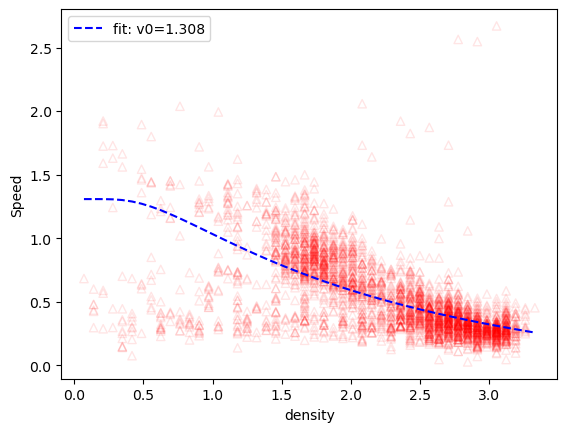
\includegraphics[width=0.4\textwidth]{images/t3_curvefit_bn_dens.png}}
\subfigure[Corridor]{
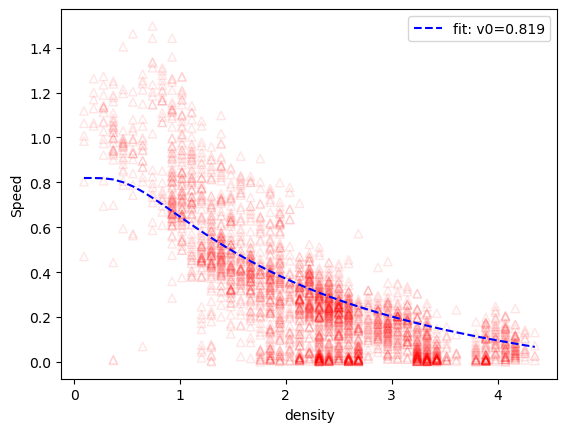
\includegraphics[width=0.4\textwidth]{images/t3_curvefit_cd_dens.png}}
\caption{Curve fitting $v_0$ on the densities}
\label{fig:cv_dens}
\end{figure}

\begin{table}[H]
\centering
\begin{tabular}{ |c|c|c| }
\hline
Scenario & $v_0$ (our) & $v_0$ (paper)\\
\hline
Bottleneck & $1.308$ & $1.64$\\
\hline
Corridor & $0.819$ & $1.50$\\
\hline
\end{tabular}
\caption{$v_0$ from curve fitting density}
\label{Tab:v0dens}
\end{table}

To double-check if curve-fitting on the original Weidemann model was meaningful, we next perform curve-fitting once again using the obtained $v_0$. Additionally as previously mentioned we use the fixed physical size $l=0.625$. Now we are left with obtaining the parameter $T$. In figure \ref{fig:cv_og} we plotted the results after curve-fitting. This plot is similar to the one from the paper \cite{tordeux2020prediction} figure 4. In table \ref{Tab:tdens} we see that our results for the parameter $T$  are quite similar to the one from the paper.

\begin{figure}[H]
\centering
\subfigure[Bottleneck]{
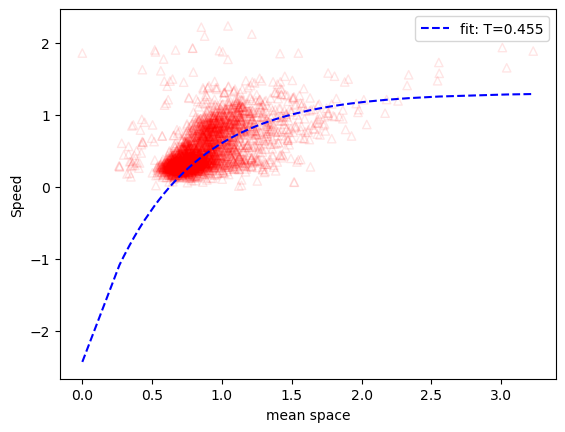
\includegraphics[width=0.4\textwidth]{images/t3_curvefit_bn_og.png}}
\subfigure[Corridor]{
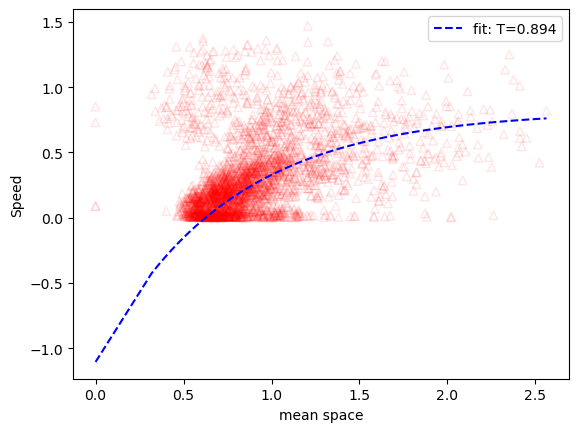
\includegraphics[width=0.4\textwidth]{images/t3_curvefit_cd_og.png}}
\caption{Curve fitting $T$ on original Weidmann function}
\label{fig:cv_og}
\end{figure}

\begin{table}[H]
\centering
\begin{tabular}{ |c|c|c| }
\hline
Scenario & $T$ (our) & $T$ (paper)\\
\hline
Bottleneck & $0.455$ & $0.49$\\
\hline
Corridor & $0.894$ & $0.85$\\
\hline
\end{tabular}
\caption{$T$ from curve fitting original Weidmann function}
\label{Tab:tdens}
\end{table}

\paragraph{3}
Since curve-fitting can be performed on multiple parameters simultaneously, we will next try to obtain the parameter $v_0$ and $T$ given $l=0.625$. In figure \ref{fig:cv} we see the resulting values for $v_0$ and $T$. In tables \ref{Tab:v0cv} and \ref{Tab:v0cv1} we see that our results for speed are now closer to the ones in the paper. At the same time the results confirm that the corridor has a much lower speed for a pedestrian in a free situation. As for the parameter $T$ in table \ref{Tab:tcv} the values are still similar to the results from the paper, though for the corridor scenario $T$ has a much higher value compared to the result obtained from the previous section.

\begin{figure}[H]
\centering
\subfigure[Bottleneck]{
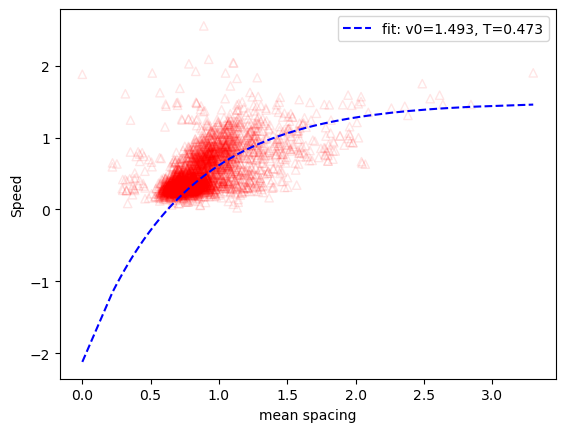
\includegraphics[width=0.4\textwidth]{images/t3_curvefit_bn.png}}
\subfigure[Corridor]{
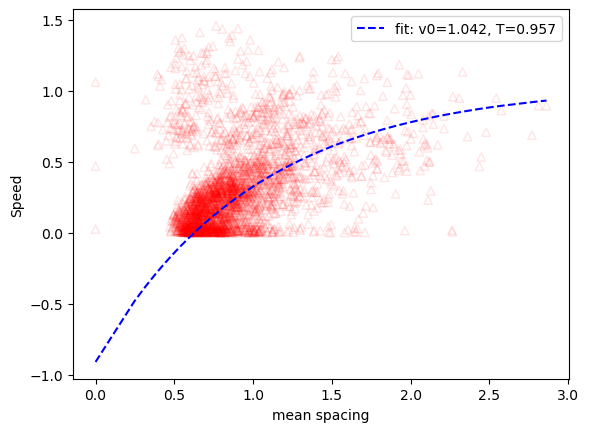
\includegraphics[width=0.4\textwidth]{images/t3_curvefit_cd.png}}
\caption{Curve fitting $T$ on original Weidmann function}
\label{fig:cv}
\end{figure}

\begin{table}[H]
\centering
\begin{tabular}{ |c|c|c| }
\hline
Scenario & $v_0$ (our) & $v_0$ (paper)\\
\hline
Bottleneck & $1.493$ & $1.64$\\
\hline
Corridor & $1.042$ & $1.50$\\
\hline
\end{tabular}
\caption{$v_0$ from curve fitting equation \ref{exp_tor}}
\label{Tab:v0cv}
\end{table}

\begin{table}[H]
\centering
\begin{tabular}{ |c|c|c| }
\hline
Scenario & $T$ (our) & $T$ (paper)\\
\hline
Bottleneck & $0.473$ & $0.49$\\
\hline
Corridor & $0.957$ & $0.85$\\
\hline
\end{tabular}
\caption{$T$ from curve fitting on equation \ref{exp_tor}}
\label{Tab:tcv}
\end{table}

As our final test we are curve-fitting the parameter $v_0$ given $T, l$ from the paper \cite{tordeux2020prediction} in table 1. In figure \ref{fig:cv_pap} we can see similar results as seen from previous tests. Compared to the results from curve-fitting on 2 parameters here $v_0$ has a higher speed in the bottleneck scenario and lower speed the corridor case. Overall the results are similar to the tests performed previously.

\begin{figure}[H]
\centering
\subfigure[Bottleneck]{
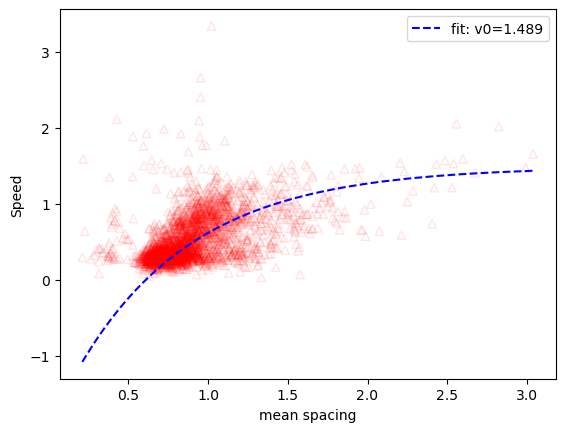
\includegraphics[width=0.4\textwidth]{images/t3_curvefit_bn_pap.png}}
\subfigure[Corridor]{
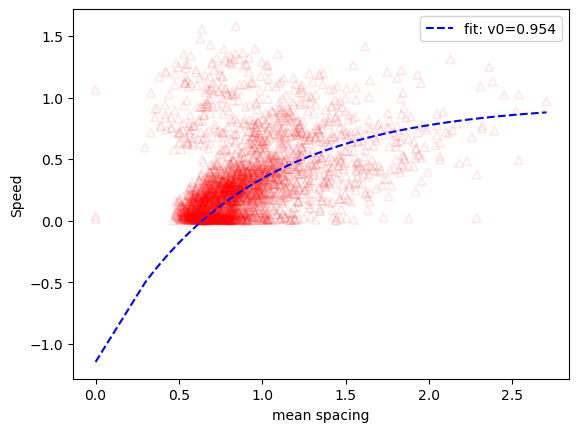
\includegraphics[width=0.4\textwidth]{images/t3_curvefit_cd_pap.png}}
\caption{Curve fitting $v_0$ on original Weidmann function}
\label{fig:cv_pap}
\end{figure}

\begin{table}[H]
\centering
\begin{tabular}{ |c|c|c| }
\hline
Scenario & $v_0$ (our) & $v_0$ (paper)\\
\hline
Bottleneck & $1.549$ & $1.64$\\
\hline
Corridor & $0.923$ & $1.50$\\
\hline
\end{tabular}
\caption{$v_0$ from curve fitting equation \ref{exp_tor}}
\label{Tab:v0cv1}
\end{table}

\paragraph{Conclusion}
Overall we can obtain similar results for the parameter $T$. As for the parameter $v_0$ we can have similar results for the bottleneck scenario, but for the corridor scenario we have significantly lower values. This is likely due to different ways of preprocessing data, as it is not specified in the paper itself. But we could still say that relatively speaking, we can draw the a similar conclusion, since $v_0$ is higher in the bottleneck case compared to the corridor case.

In table \ref{Tab:v0complete} we see a final comparison the results from all approaches. Overall all results show that $v_0$ has a higher value for the Bottleneck scenario than the corridor scenario. In this case approach (1) is closer the results in the paper in terms of its ratio. We can conclude that our data processing approach is probably incomplete, as the pedestrian speed in a free situation $v_0$ shouldn't be too different between both scenarios.

\begin{table}[H]
\centering
\begin{tabular}{ |l|c|c|c| }
\hline
Scenario & Bottleneck & Corridor & Ratio ($B/C$)\\
\hline
$v_0$ from paper & $1.64$ & $1.50$ & $1.093$\\
\hline
$v_0$ from (1) & $1.009$ & $0.787$ & $1.282$\\
\hline
$v_0$ from (2) & $1.308$ & $0.819$ & $1.597$\\
\hline
$v_0$ from (3.1) & $1.493$ & $1.042$ & $1.433$\\
\hline
$v_0$ from (3.2) & $1.549$ & $0.923$ & $1.678$\\
\hline
\end{tabular}
\caption{$v_0$ from all approaches}
\label{Tab:v0complete}
\end{table}

\end{task}